%%%%%%%%%% Page 1 - Col 1 %%%%%%%%%%
\newpage
\colorfulheader{computer science}

\begin{minipage}[t]{0.485\textwidth}
    \textbf{Bit Manipulation}
    \begin{customcenter}[4pt]
        \begin{tabular}{|c|c|c|c|c|c|}
             \hline
             \texttt{x} & \texttt{y} & \texttt{x \& y} & \texttt{x | y}& \texttt{x \string^ y} & {\raisebox{1.5pt}{\texttildelow}}\texttt{x} \\
             \hline
             1 & 1 & 1 & 1 & 0 & 0 \\
             \hline
             1 & 0 & 0 & 1 & 1 & 0 \\
             \hline
             0 & 1 & 0 & 1 & 1 & 1 \\
             \hline
             0 & 0 & 0 & 0 & 0 & 1 \\
             \hline
        \end{tabular}
    \end{customcenter}
    \textbf{Data Structures}
    \begin{itemize}
        \setlength\itemsep{0pt}
        \item A \textbf{linked list} can be implemented as \\ 
        {singly} \inlinecode{1->2->3->NULL} \\ 
        {doubly} \inlinecode{NULL<-1<->2<->3->NULL} \\ 
        {circular} \inlinecode{1->2->3->1} or \inlinecode{1<->2<->3<->1} 
        \item The \textbf{queue} can be done \textbf{circular}. The $n + 1$ element is inserted in the $0$ index if it is empty
        \item A \textbf{binary tree} (sometimes named only tree) is a hierarchical data structure that has \textbf{at most} 2 children
        \item Representation for binary tree is \\ 
        1. Data \inlinecode{node->data} \\ 
        2. Pointer to left child \inlinecode{node->left} \\ 
        3. Pointer to right child \inlinecode{node->right} 
        \item Traversing a binary tree can be done as \\ 
        \textbf{Depth First} \\
        \textcolor{white}{\hspace{2em}} Inorder (Left-Root-Right) \\
        \textcolor{white}{\hspace{2em}} Preorder (Root-Left-Right) \\
        \textcolor{white}{\hspace{2em}} Postorder (Left-Right-Root) \\ 
        \textbf{Breadth First} \\
        \textcolor{white}{\hspace{2em}} Level order
        \item Maximum number of nodes of tree at level $l$ is $2^l$
        \item For a tree of height $h$, the maximum number of nodes is $2^{\parenthesisA{h + 1}} - 1$
        \item If not balanced the traversal complexity of a tree if height $h$ can be $O\parenthesisA{h}$
        \item A \textbf{binary search tree} (bst) has the following properties \\
        1. For each left subtree $\text{node}_l^{\text{value}} < \text{node}^{\text{value}}$\\
        2. For each right subtree has $\text{node}_r^{\text{value}} > \text{node}^{\text{value}}$\\
        3. The left and right subtree are also a bst
        \item A \textbf{graph} consist of \\ 
        1. Finite set of vertices called \textbf{nodes} \\ 
        2. Finite set of ordered pairs $\parenthesisA{u_i, v_j}$ called \textbf{edges} \\ \bracket{Directed graphs have $\parenthesisA{u_i, v_j}\neq\parenthesisA{v_j, u_i}$} \\ 
        3. An edge may contain a \textbf{weight} (also named value or cost)
        \item For graphs it is common to represent \\ 
        $V\mapsto\text{Number of vertices}$ \\
        $E\mapsto\text{Number of edges}$
        \item Graphs can be implemented as an \textbf{adjacency matrix} or as an \textbf{adjacency list}, having the following properties
        \begin{center}
        \begin{tabular}{|c|c|c|}
        \hline
             \textbf{Graph Implementation} & \textbf{Traversal} & \textbf{Space}  \\
        \hline
             Matrix & $O\parenthesisA{V^2}$ & $O\parenthesisA{V^2}$ \\
        \hline
             List & $O\parenthesisA{V + E}$ & $O\parenthesisA{V + E}$ \\
        \hline
        \end{tabular}
        \end{center}
    \end{itemize}
\end{minipage}
%%%%%%%%%%%%%%%%%%%%%%%%%%%%%%%%%%%%
\hspace{5pt}
%%%%%%%%%% Page 1 - Col 2 %%%%%%%%%%
\begin{minipage}[t]{0.485\textwidth}
    For example, given the following graph
    \begin{customcenter}[2pt]
        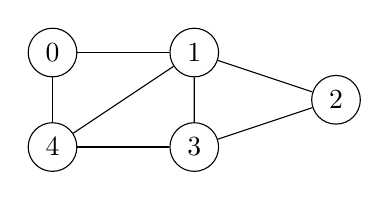
\begin{tikzpicture}[x=1cm, y=1cm, xscale=0.6, yscale=0.6, baseline=5.5pt]
        \node[circle, draw, minimum size=10pt] (c0) at (0,0){0}; 
        \node[circle, draw, minimum size=10pt] (c1) at (3,0){1}; 
        \node[circle, draw, minimum size=10pt] (c2) at (6,-1){2}; 
        \node[circle, draw, minimum size=10pt] (c3) at (3,-2){3}; 
        \node[circle, draw, minimum size=10pt] (c4) at (0,-2){4};
        \draw (c0) -- (c1);
        \draw (c0) -- (c4);
        \draw (c1) -- (c3);
        \draw (c4) -- (c1);
        \draw (c1) -- (c2);
        \draw (c2) -- (c3);
        \draw (c4) -- (c3);
        \end{tikzpicture}
    \end{customcenter}
    Can be represented as the matrix (right) or the list (left)\\
    \begin{minipage}[t]{0.485\textwidth}
        \vfill
        \centering
        \begin{tabular}{|c|ccccc|}
        \hline
        {} & 0 & 1 & 2 & 3 & 4 \\
        \hline
         0 & 0 & 1 & 0 & 0 & 1 \\
         1 & 1 & 0 & 1 & 1 & 1 \\
         2 & 0 & 1 & 0 & 1 & 0 \\
         3 & 0 & 1 & 1 & 0 & 1 \\
         4 & 1 & 1 & 0 & 1 & 0 \\
        \hline
        \end{tabular}
        \vfill
    \end{minipage}
    \begin{minipage}[t]{0.485\textwidth}
        \vfill
        \centering
        \begin{lstlisting}
            0 [] -> 1 [] -> 4 []
            1 [] -> 2 [] -> 3 [] -> 4 []
            2 [] -> 1 [] -> 3 []
            3 [] -> 1 [] -> 2 [] -> 4 []
            4 [] -> 3 [] -> 1 [] -> 0 []
        \end{lstlisting}
        \vfill
    \end{minipage}
    \emptyline
    \emptyline
    \textbf{C Memory Layout}
    \begin{itemize}
        \setlength\itemsep{0pt}
        \item Consists \quotes{typically} of 5 sections: 1. Text segment, 2. Initialized data segment, 3. Uninitialized data segment, 4. Heap, and 5. Stack
        \item The \textbf{text segment} contains the executable instructions. Can be places below the heap or stack regions. It is \textbf{read-only}
        \item \textbf{Initialized data segment} (or simply data segment) contains \textbf{global} and \textbf{static} variables \textbf{initialized by the programmer}. It can be subdivided in \textbf{read-only} and \textbf{read-write} areas. The following are examples of data segment \\ 
        \textcolor{white}{\hspace{1em}}\inlinecode{static int n = 10;}\\
        \textcolor{white}{\hspace{1em}}(defined anywhere)\\
        \textcolor{white}{\hspace{1em}}\inlinecode{const char * string = "hello world";}\\
        \textcolor{white}{\hspace{1em}}(defined outside the \inlinecode{main} function)
        \item \textbf{Uninitialized data segment} (or \quotes{block started by symbol} $\mapsto$ bss) contains \textbf{global} and \textbf{static} variables \textbf{not initialized explicitly} or initialized to zero. The following are examples of bss segment \\ 
        \textcolor{white}{\hspace{1em}}\inlinecode{static int i;}\\
        \textcolor{white}{\hspace{1em}}(defined anywhere)\\
        \textcolor{white}{\hspace{1em}}\inlinecode{int j;}\\
        \textcolor{white}{\hspace{1em}}(defined before the \inlinecode{main} function)
        \item The \textbf{stack} area contains the program stack (LIFO data structure) located in the higher parts of the memory (on x86 architecture it grows towards address zero). A set of values pushed for one function call is defined as \textbf{stack frame} (consisting at minimum of a return address). Each call to the stack allocates room for \textbf{automatic} and \textbf{temporary} variables. Allocation happens at \textbf{function call}
        \item The \textbf{heap} segment is where dynamic memory allocation takes place. Begins at the end of the bss segment and grows to larger addresses. In \inlinecode{C} language the heap area can be managed by \inlinecode{malloc, realloc} and \inlinecode{free} functions. \quotes{Contiguous} heap region is not mandatory for the previous C functions resulting in the possibility of \textbf{memory fragmentation}. Allocation happens at \textbf{execution of instruction}
    \end{itemize}
\end{minipage}
%%%%%%%%%% Page 2 %%%%%%%%%%
\newpage
\colorfulheader{computer science}
\begin{customcenter}[0pt]
    \begin{customcenter}[2pt]
        \textbf{\textcolor{white}{\hspace{2em}}C Memory Layout Comparison}
    \end{customcenter}
    \begin{tabular}{|l|c|c|}
         \hline
         & \textbf{Stack} & \textbf{Heap} \\
         \hline
         \textbf{Memory} & Allocated in contiguous block & Allocated in any random order \\ 
         \hline
         \textbf{Allocation/Deallocation} & Automatic by compiler & Manual by programmer \\
         \hline
         \textbf{Cost} & Less & More \\
         \hline
         \textbf{Implementation} & Easy & Hard \\
         \hline
         \textbf{Access Time} & Faster & Slower \\
         \hline
         \textbf{Main Issue} & Small memory & Memory fragmentation \\
         \hline
         \textbf{Safety} & Thread safe & Not thread safe (data visible to all threads) \\
         \hline
         \textbf{Data Type} & Linear & Hierarchical \\
         \hline
    \end{tabular}
    \emptyline
    \vspace{5pt}
    \begin{customcenter}[2pt]
    \textbf{\textcolor{white}{\hspace{2em}}Data Structures Complexity}
    \end{customcenter}
    \begin{tabular}{|l|c|c|c|c|c|}
         \hline
         & Accessing & Search & Insertion & Deletion & Space \\
         \hline
         Array & \DSC{1} & \DSC{n} & \DSC{n} & \DSC{n} & \DSC{n} \\
         \hline
         Stack (LIFO) & \DSC{n} & \DSC{n} & \DSC{1} & \DSC{1} & \DSC{n} \\
         \hline
         Queue (FIFO) & \DSC{n} & \DSC{n} & \DSC{1} & \DSC{1} & \DSC{n} \\
         \hline 
         Linked List & \DSC{n} & \DSC{n} & \DSC{1} & \DSC{1} & \DSC{n} \\
         \hline
         Hash Table & & \DSC{1} & \DSC{1} & \DSC{1} & \DSC{n} \\
         \hline
         Binary Search Tree$^*$ & \DSC{h} & \DSC{h} & \DSC{h} & \DSC{h} & \DSC{n} \\
         \hline
         Binary Heap & Min Heap \DSC{1} & \DSC{log\text{ }n} & \DSC{log\text{ }n} & \DSC{log\text{ }n} & \DSC{n} \\
         & Max Heap \DSC{1} & & & & \\
         \hline
    \end{tabular}
    \\
    $^*h$ would be the height of the tree. If tree is balanced $h = log\text{ } n$
\end{customcenter}
\vspace{5pt}
%%%%%%%%%% Page 2 - Col 1 %%%%%%%%%%
\begin{minipage}[t]{0.485\textwidth}
    \textbf{Dynamic Programming}\\
    \emptyline
    Programming paradigm to \textbf{efficiently} explore all possible solutions to a problem. The problem should have one of the following characteristics
    \begin{itemize}
        \setlength\itemsep{0pt}
        \item \underline{Problem can be broken down in \textbf{overlapping subproblems}}
        
        A rule of thumb is to notice if \textbf{future decisions depend on earlier decision}        
        \item \underline{Problem has an \textbf{optimal substructure}}

        For example the problem would ask optimal value (min or max) of something, here are some sample phrases
        \begin{itemize}
            \item What is the minimum cost of...
            \item Compute the maximum profit from...
            \item How many ways can you...
            \item Find the longest possible...
        \end{itemize}
    \end{itemize}
    Care has to be taken to not confuse a dynamic programming (DP) problem with \textbf{greedy} problems. Both would have optimal substructure but greedy does not have overlapping characteristic.\\
    \emptyline
    Two ways of implementing a DP algorithm,\\ 
    \textbf{Top-Down} (recursion) or \textbf{Bottom-Up} (iterative).\\
    
    An important optimization in the top-down approach is \textbf{memoization} that stored previously computed subresults (commonly in a hash) to be re-used in the future, avoiding recomputation.
    \begin{customcenter}[8pt]
        \begin{tabular}{|c|c|c|}
            \hline
            & \textbf{Top-Down} & \textbf{Bottom-Up} \\
            \hline
            Pro & Easy to write & Runs faster\\
            \hline
            Con & Overhead & Order of operations matter\\
            \hline
        \end{tabular}
    \end{customcenter}
    In DP one can define a \textbf{state} as a \textbf{set of variables that can sufficiently describe a scenario}.
\end{minipage}
%%%%%%%%%%%%%%%%%%%%%%%%%%%%%%%%%%%%
\hspace{5pt}
%%%%%%%%%% Page 2 - Col 2 %%%%%%%%%%
\begin{minipage}[t]{0.485\textwidth}
    To \quotes{\textit{produce}} an algorithm for a DP problem, one can follow the next steps:
    \begin{enumerate}
        \setlength\itemsep{0pt}
        \item Create a \textbf{function} or \textbf{data structure} that will compute the answer of the problem for \textbf{every given state}
        \item A \textbf{recurrence relation} to transition between states
        \item Define \textbf{bases cases} to avoid inifinite recursion or faulty iterations
    \end{enumerate}
    For example, the following \textbf{climbing stairs} problem
    \begin{tcolorbox}
        You are climbing a staircase. It takes $n$ steps to reach the top. Each time you can either climb $1$ or $2$ steps. \textbf{How many distinct ways} can you climb to the top?
    \end{tcolorbox}

    Thus, the DP steps for above problem would be
    \begin{enumerate}
        \setlength\itemsep{0pt}
        \item \textbf{Function} $dp(i)$, where $i$ represents how many ways to climb to the $i^{\text{th}}$ step.
        \item \textbf{Recurrence} $dp(i) = dp(i - 1) + dp(i - 2)$, since according to the description one can climb either $1$ or $2$ steps each time.
        \item \textbf{Base Case} $dp(1) = 1$ and $dp(2) = 2$, since there is 1 way (1 step) to climb to step 1 and 2 ways (1 step + 1 step and 2 step) to climb to step 2.
    \end{enumerate}
    A minimal implementation in C\texttt{++} of above steps is
    \begin{lstlisting}
        int dpRecursive(int i)
        {
            if (i <= 2) return i; // base case
            // recurrence
            return dpRecursive(i - 1) + dpRecursive(i - 2);
        }
        int countSteps(int n) { return dpRecursive(n); }
    \end{lstlisting}
    Although the code would solve the problem, it has poor complexities, $\mathcal{O}\parenthesisA{2^n}$ time and $\mathcal{O}\parenthesisA{n}$ space.
\end{minipage}

%%%%%%%%%% Page 3 - Col 1 %%%%%%%%%%
\newpage
\colorfulheader{computer science}

\begin{minipage}[t]{0.485\textwidth}
    To improve time complexity, \textbf{memoization} is required
    \begin{lstlisting}
        unordered_map<int,int> memo;
        int dpRecursiveWithMemo(int i)
        {
            if (i <= 2) return i; // base case
            if (memo.find(i) == memo.end())
            {
                // recurrence
                memo[i] = dpRecursive(i - 1) + dpRecursive(i - 2);
            }
            return memo[i];
        }
        int countSteps(int n) { return dpRecursiveWithMemo(n); }
    \end{lstlisting}
    Which converts the time complexity to $\mathcal{O}\parenthesisA{n}$.\\

    One can also change the above \textbf{Top-Down} to a \textbf{Bottom-Up} implementation. The key for it is just to modify the recursion for an iteration while preserving the 3 steps to solve a DP problem, i.e.
    \begin{enumerate}
        \setlength\itemsep{0pt}
        \item \textbf{Data Structure} \texttt{dp[i]}, where \texttt{dp} is an array
        \item \textbf{Recurrence} \texttt{dp[i] = dp[i - 1] + dp[i - 2]}
        \item \textbf{Base Case} \texttt{dp[1] = 1}, \texttt{dp[2] = 2}
    \end{enumerate}
    Thus, an implementation of the bottom-up version would be
    \begin{lstlisting}
        int countSteps(int n)
        {
            if (n <= 2) return n;
            vector<int> dp(n + 1, 0); // data structure
            dp[1] = 1; // base case
            dp[2] = 2; // base case
            for (int i = 3; i <= n; i++)
            {
                dp[i] = dp[i - 1] + dp[i - 2]; // recurrence
            }
            return dp[n];
        }
    \end{lstlisting}
    Notice how for this problem \texttt{dp} requires to be of length $n + 1$. This implementation would have the same complexities as before, i.e. $\mathcal{O}\parenthesisA{n}$ for time and space.\\

    Lastly, one can improve the space complexity to be constant by noticing that at each step the iterative approach only cares about the \textbf{previous 2 steps}. Therefore, removing the array \texttt{dp} the \textbf{optimized solution for the climbing stairs problem is}
    \begin{lstlisting}
        int countStepsOptimized(int n)
        {
            if (n <= 2) return n;
            step1 = 1; // base case
            step2 = 2; // base case
            for (int i = 3; i <= n; i++)
            {
                int nextStep = (step1 + step2); // recurrence
                step1 = step2;
                step2 = nextStep;
            }
            return step2;
        }
    \end{lstlisting}
    Which makes a $\mathcal{O}\parenthesisA{1}$ space complexity.
\end{minipage}